\documentclass[11pt, oneside]{article}   	% use "amsart" instead of "article" for AMSLaTeX format
\usepackage{geometry}                		% See geometry.pdf to learn the layout options. There are lots.
\geometry{letterpaper}                   		% ... or a4paper or a5paper or ... 
%\geometry{landscape}                		% Activate for for rotated page geometry
%\usepackage[parfill]{parskip}    		% Activate to begin paragraphs with an empty line rather than an indent
\usepackage{graphicx}				% Use pdf, png, jpg, or eps� with pdflatex; use eps in DVI mode
								% TeX will automatically convert eps --> pdf in pdflatex		
\usepackage{amssymb}
\usepackage{amsmath}
\usepackage{parskip}
\usepackage{color}
\usepackage{hyperref}

\title{Charles's birdhouse}
%\author{The Author}
%\section{}
%\subsection*{}
\date{}							% Activate to display a given date or no date

\graphicspath{{/Users/telliott_admin/Dropbox/Tex/png/}}
% \begin{center} 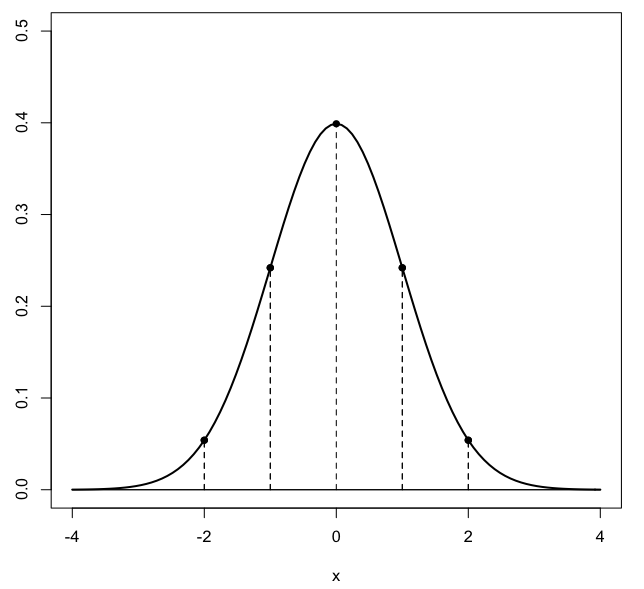
\includegraphics [scale=0.4] {gauss3.png} \end{center}
\begin{document}
\maketitle
\Large
Suppose we are constructing a dormer on a roof.  Here is the main roof.  
\begin{center} 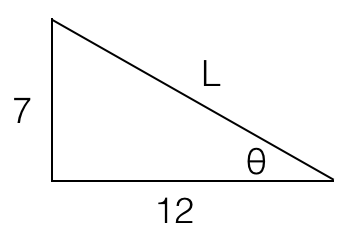
\includegraphics [scale=0.5] {birdhouse1.png} \end{center}
The pitch of a roof is usually given as rise over run (e.g. 7 in 12 or 7/12).  We can calculate the length of the third side (the hypotenuse) using Pythagoras
\[ 7^2 + 12^2 = L^2 \]
$L = 14.07$.  or we can say that $7/12$ is the tangent of the angle $\theta$.
\[ \tan \theta = 7/12 = 0.583 \]
\[ \theta = \tan^{-1} 0.583 = 0.528 \]
That's in radians.  To convert to degrees, multiply by 57.3 (degrees per radian).
\[ \theta = 0.528 \times 57.3 = 30.25 \]
which seems correct since if $L$ were exactly twice $7$, then the angle would be exactly $30$ degrees.
\subsection*{dormer}
\begin{center} 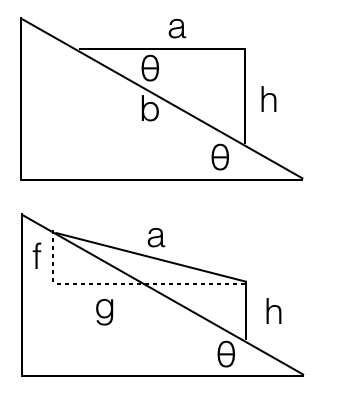
\includegraphics [scale=0.5] {birdhouse2.png} \end{center}
Now for the dormer.  Although we might possibly have a dormer that has a horizontal ridge, the more general case does not.  So we choose the dimensions of the dormer as, say
\begin{itemize}
\item the lowest point on the roof
\item the highest point on the roof
\item the height of the dormer, $h$
\end{itemize}

Then we know the dimensions $a$, $g$, $f$.  If you want we could calculate them based on $\theta$, $h$ and the angle of the dormer, but I assume it is more natural to pick $f$ and $g$ or the high and low points on the roof, than to determine the exact angle of the dormer roof.

We also need a shape for the profile of the dormer.  For example, we might choose $c$ = $h$ in the figure below.  This determines $d$, using Pythagoras.
\begin{center} 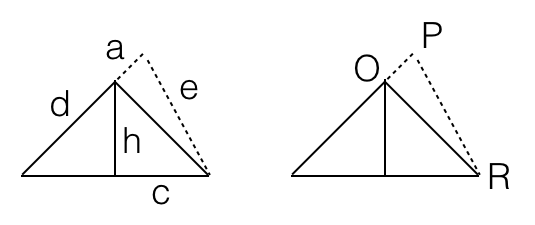
\includegraphics [scale=0.5] {birdhouse3.png} \end{center}

At this point, we want to calculate the shape of the decking of the dormer roof.  We are assuming that we have two of the sides $a$, and $d$, based on what we've said so far.  We do not know the third side, $e$, nor do we know any of the angles.
\begin{center} 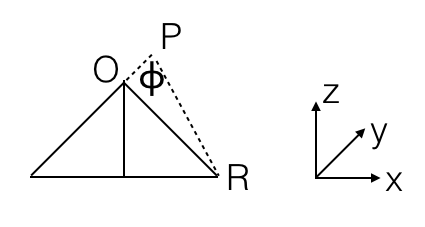
\includegraphics [scale=0.5] {birdhouse6.png} \end{center}

One way to approach this is using vectors.  If we choose the origin $O$ as shown and $x,y,z$ oriented in the usual way, then we can write:
\[ \mathbf{OR} = \ \langle \ c,0,-h \ \rangle \]
\[ \mathbf{OP} = \ \langle \ 0,g,f  \ \rangle \]
\[ \mathbf{PR} = \ \langle \ c,-g,-(f+h)  \ \rangle \]
So then the lengths are easily calculated, e.g.
\[ d^2 = | \mathbf{OR} |^2 = c^2 + h^2 \]
\[ a^2 = | \mathbf{OP} |^2 = g^2 + f^2 \]
We don't need vectors for these first two, we can get them from Pythagoras.  But notice \[ e^2 = | \mathbf{PR} |^2 = c^2 + g^2 + (f+h)^2 \]
\[ = a^2 + d^2 + 2fh \]
It cannot be an accident that this is almost Pythagoras (the triangle we are interested in has sides $a$,$d$,$e$ but is not a right triangle), and $f+h$ is the height of the dormer.  We will see later why this works.

An alternative method to calculate the distance $e$ squared is to find the total displacement in each of the three directions between $P$ and $R$, square each of those and add them (which is just saying find the length of the vector in other language).
\[ \Delta x = c \]
\[ \Delta y = g \]
\[ \Delta z = h + f \]
Summing the squares:
\[ e^2 = \Delta x^2 + \Delta y^2 + \Delta z^2 \]
\[ = c^2 + g^2 + (h+f)^2 \]
\[ = c^2 + g^2 + h^2 + 2hf + f^2 \]
but $g^2  = a^2 - f^2$
\[ e^2 = c^2 + a^2 - f^2 + h^2 + 2hf + f^2 \]
\[ = c^2 + a^2 + h^2 + 2hf \]
and $h^2 = d^2 - c^2$
\[ e^2 = c^2 + a^2 + d^2 - c^2 + 2hf \]
\[ = a^2 + d^2 + 2hf \]
And that is the same is what we had above.
Recall what $a$, $f$ and $h$ are:
\begin{center} 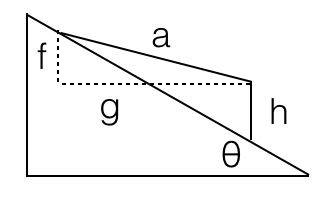
\includegraphics [scale=0.5] {birdhouse4.png} \end{center}

So now we have $e^2$ and thus $e$.  

Practically speaking we could just stop here, knowing all three sides $a$,$d$ and $e$.  We lay out the triangle with a pair of dividers or a big meter stick, and just cut it.

But we set up the vectors in order to use the properties of the \emph{dot product}.  

We labeled the vertices $O$, $P$,$R$ as shown.  If the angle at vertex $P$ is labeled as $\phi$
\begin{center} 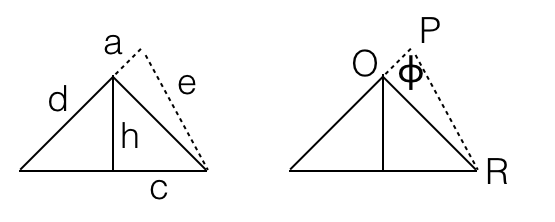
\includegraphics [scale=0.5] {birdhouse5.png} \end{center}
The dot product of two vectors is equal to the product of the length of each vector times the cosine of the angle between them.

The dot product is
\[  \mathbf{PR} \cdot \mathbf{PO} = \mathbf{PR} \cdot (-\mathbf{OP}) \]
\[ = \ \langle \ 0,g,f  \ \rangle \cdot - \langle \ c,-g,-(f+h)  \ \rangle \]
\[ = g^2 + f(f+h) \]
and that is equal to the product of the length of each vector times the cosine of the angle between them
\[ ae \cos \phi \]

So
\[ \cos \phi = \frac{g^2 + f^2 + fh }{a e} \]
and a similar computation can be made for any angle of the triangle.

\subsection*{law of cosines}
An alternative formulation that uses the lengths of the sides is the law of cosines, which says that if vertex $\phi$ is the angle opposite side $d$ while the other two sides $a$ and $e$ flank angle $\phi$, then
\[ d^2 = a^2 + e^2 - 2ae \cos \phi \]
\[ \cos \phi = \frac{a^2 + e^2 - d^2}{2ae} \]
(If $\phi$ were $90$ degrees this would be Pythagoras).

Compared to what we had before:
\[ \cos \phi = \frac{g^2 + f^2 + fh }{a e} \]
For these to be equivalent statements we must show that
\[ 2(g^2 + f^2 + fh) = a^2 + e^2 - d^2 \]
Let's start with the right-hand side
\[ a^2 + e^2 - d^2 \]
we can substitute $e^2 = a^2 + d^2 + 2hf$ from before so we have
\[ 2a^2 + d^2 + 2hf - d^2 \]
\[ =  2a^2 + 2hf  \]
and $f^2 + g^2  = a^2$ so
\[ = 2(g^2 + f^2) + 2hf \]
Looks like we did it!  These are equivalent computations:

\[ \cos \phi = \frac{a^2 + e^2 - d^2}{2ae} \]
\[ \cos \phi = \frac{g^2 + f^2 + fh }{a e} = \frac{a^2 + fh}{ae} \]
\begin{center} 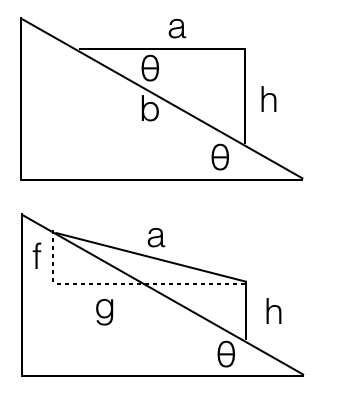
\includegraphics [scale=0.5] {birdhouse2.png} \end{center}
\begin{center} 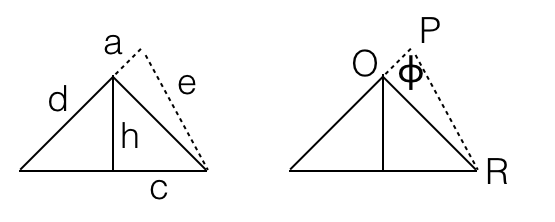
\includegraphics [scale=0.5] {birdhouse5.png} \end{center}



\end{document}  